\documentclass[mathserif]{beamer}
\usepackage{amsmath}
\usepackage{graphicx}
\usetheme{Frankfurt}

\title{Interference Temperature}
\author{Swrangsar Basumatary \\
\texttt{swrangsar@iitb.ac.in}}
\institute{Department of Electrical Engineering \\ Indian Institute of Technology Bombay}
\date{April 2013}
\begin{document}



\frame{\titlepage}



\begin{frame}{Introduction}

\begin{itemize}
	\pause
	\item The concept of interference temperature was introduced by the FCC as a new metric for quantifying and managing interference.
	\pause
	\item Using this model, \emph{Cognitive Radios} operating in licensed frequency bands would be able to measure their current interference environment and adjust their transmission characteristics so as not to raise the interference temperature over a limit set by the regulators.
\end{itemize}

\end{frame}



\begin{frame}{Purpose of the metric}

\begin{itemize}
	\pause 
	\item \textbf{The purpose of this metric is to remove the subjective context that has been the basis of interference analysis up to now.}
	\pause
	\item Currently, they do a  detailed analysis of the surroundings and rely on worst case analysis.
	
	
	\item But relying on worst case analysis leaves much of the spectrum unused. 
\end{itemize}

\end{frame}



\begin{frame}{Driving forces for interference metric}

\begin{itemize}
\pause
\item \textbf{Changing landscape} \\

Technological advances have led to increased diversity of spectrum-based consumer applications. This has resulted in an increased demand for spectral resources. Static interference management does not work anymore.

\pause
\item \textbf{Increased density and mobility} \\

People are owning more cellular devices. Density of mobile devices has increased and interference management has become more complicated.

\end{itemize}

\end{frame}



\begin{frame}{Definition of Interference Temperature}

Interference temperature, $T_I$ is defined as
\begin{equation*} 
    T_I(f_c , B) = \frac{P_I(f_c , B)}{kB}
\end{equation*}

where 

\begin{itemize}
	\item $P_I(f_c,B)$ is the average interference power centered at frequency, $f_c$, and covering bandwidth
$B$. 
	\item $k$ is the Boltzmann's constant $k = 1.38 \times 10^{-23} J/K $ 
\end{itemize}

\pause
In SI system, the unit of interference temperature turns out to be \emph{degrees Kelvin}.

\end{frame}



\begin{frame}{Interference Temperature Models}

There is ambiguity regarding whether to represent $T_I$ in terms of the transmitter parameters or the receiver parameters. This results into two models \footnote{T. Charles Clancy, \emph{Formalizing the Interference Temperature Model}. Wiley Journal On Wireless Communications And Mobile Computing, 2006.}:

\pause
\begin{enumerate}
    \item Ideal model
    \item Generalized model \\~\\
\end{enumerate}
\end{frame}



\begin{frame}{IT model figures}

\begin{figure}[p]
\centering
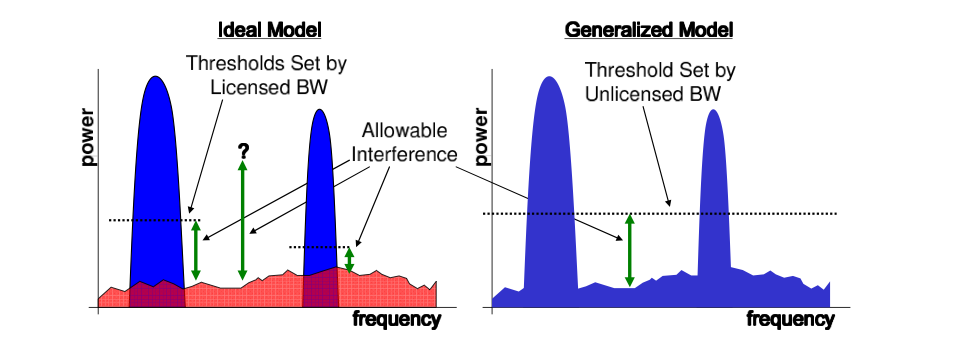
\includegraphics[width = \linewidth]{interferenceTemperatureModels.png}
\caption{Ideal and Generalized interpretations of the Interference Temperature Model. (Source: T. Charles Clancy, \emph{Formalizing the Interference Temperature Model}, Wiley Journal On Wireless Communications And Mobile Computing, 2006.)}
\end{figure}

\end{frame}




\begin{frame}{Ideal model}

In the ideal model we try to guarantee that
\begin{equation}
    T_I(f_i,B_i) + \frac{M_iP}{kB_i} \leq T_L(f_i) \qquad \forall \quad 1 \leq i \leq n \label{idealModel}
\end{equation}
where

\pause
\begin{itemize}
	
	\item $T_I(f_i,B_i)$ is  the interference temperature of the $i$'th receiver with center frequency $f_i$ and bandwidth $B_i$
	\item $P$ is the power of the unlicensed transmitter
	\item $M_i$ is a constant between 0 and 1 representing the attenuation of the  transmitted power $P$ at the $i$'th receiver, and
	\item $T_L(f_i)$ is the interference temperature limit of the $i$'th receiver at center frequency $f_i$.
\end{itemize}

\pause
Usually, a unified factor $M$ (set by regulators) is used instead of $M_i$'s because we do not know the distance of every receiver. \end{frame}




\begin{frame}{Challenges in implementing the ideal model}

\begin{itemize}
    \item Hard to differentiate between licensed and unlicensed signals unless we already know the coexisting transmitters in the surrounding environment.
    \item Difficult to measure the interference temperature $T_I$ in the presence of a licensed signal. \begin{itemize}
    \item We can determine the noise floor only if the signal power goes to zero periodically. For that we have to know when the signal power is going to be zero.
    \item The other way is to take an average of the noise floor just outside the licensed signal band, but we need to have information about the licensed signal's properties, like center frequency and bandwidth.
    \end{itemize}
\end{itemize}

\end{frame}





\begin{frame}{Generalized model}

The generalized model assumes that we have no a priori knowledge about the signal environment. Thus the constraint in this model has to be written in terms of the unlicensed transmitter's parameters.
\begin{equation}
    T_I(f_c,B) + \frac{MP}{kB} \leq T_L(f_c) \label{generalizedModel}
\end{equation}
where
\pause
\begin{itemize}
	\item $T_L(f_c)$ is the interference temperature limit of the unlicensed transmitter,
	\item $T_I(f_c,B)$ is the interference temperature of the unlicensed transmitter, 
	\item $P$ is the power of the unlicensed transmitter, and
	\item $M$ is a constant between 0 and 1 representing the factor by which the transmitted power gets attenuated.
\end{itemize}

\end{frame}





\begin{frame}{Generalized model (continued)}

\begin{itemize}
\item If we constrain the transmitted power $P$ to be less than that in the ideal model, from the equations \eqref{idealModel} and \eqref{generalizedModel} we have,
\begin{equation*}
    B(T_L - T_I(f_c,B)) \leq  B_i(T_L - T_I(f_i,B_i)) \qquad \forall \quad 1 \leq i \leq n \label{powerCompare}
\end{equation*}
If every receiver receives a power $P_i$ and if the noise floor is the thermal noise temperature $T_N$, then we can rewrite the above equation as,
\begin{align*}
    kBT_L(f_c)(B-B_i) + kBT_N\sum_{j=1}^{N}B_j & \leq \sum_{j=1}^{N}B_jP_j \qquad \forall \quad 1 \leq i\leq n
\end{align*}

\pause
\item
Though $T_I(f_c,B)$ can be measured easily, inclusion of all signals in its measurement gives rise to a more complex interference environment.

\end{itemize}

\end{frame}





\begin{frame}{Properties of Interference Temperature}

\emph{The problem with Interference Temperature model is that it is too simple}. It tries to quantify interference assuming it to behave like noise. But interference doesn't actually behave like noise because we have defined interference to include all signals other than the one from the licensed transmitter. Thus, \emph{Interference Temperature} can't model interference well enough.

\end{frame}




\begin{frame}{Spectrum sensing of radio signals}


\begin{itemize}

	\pause
	\item The stimuli generated by radio emitters are non-stationary signals that depend on both time and space.
	\pause
	\item Statistical analysis of non-stationary signals is complicated and cannot be implemented efficiently in practice. 
	\pause
	\item Usually the incoming RF stimuli are sectioned into a continuous sequence of successive bursts, with each burst being short enough to justify pseudo-stationarity and yet long enough to produce an accurate spectral estimate.
	\pause
	\item A nonparametric spectral estimation method is required for this purpose and \emph{multi-taper spectral estimation} turns out to be the best choice\footnote{Simon Haykin, David J Thomson and Jeffrey H Reed, \emph{Spectrum Sensing for Cognitive Radio}, Proceedings of the IEEE, Vol. 97, No. 5, May 2009.}. 
	\pause
	\item Multitaper spectral estimation has a nice property of allowing both reduced bias and reduced variance at the same time.

\end{itemize}
\end{frame}




\begin{frame}{Multi-taper spectral estimation}
\textbf{This method uses \emph{multiple orthonormal tapers} to give different estimates of the spectrum}. These estimates are averaged to give the final estimate. \\~\\


For a time series $\{x_t\}_{t=1}^N$, the multi-taper spectral estimation procedure determines two things:
\begin{enumerate}
    \item $K$ orthonormal slepian tapers denoted by $\{w_t^{(k)}\}_{t=1}^{N}$
    \item The respective eigenspectra for each of the $K$ tapers
\begin{equation*}
   Y_k(f) = \sum_{t=1}^N w_t^{(k)} x(t) e^{-j2\pi{}ft}, \qquad k = 0, 1, ...K-1
\end{equation*}
\end{enumerate}

\end{frame}




\begin{frame}{Multi-taper spectral estimation(image)}
\begin{figure}[p]
\centering
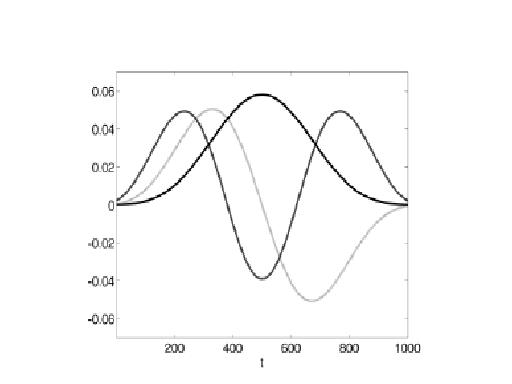
\includegraphics[height=0.65\textheight]{DPSS_figure.jpg}
\caption{The three leading Slepian sequences for T=1000 and 2WT=6. Note that each higher order sequence has an extra zero crossing. [Source: http://en.wikipedia.org/wiki/Multitaper]}
\end{figure}

\end{frame}




\begin{frame}{Multi-taper spectral estimation(continued)}

\begin{itemize}

	\item Most of the energy of the eigenspectra remain confined inside the \emph{resolution bandwidth}, denoted by $2W$ i.e. between $f-W$ and $f+W$. The \emph{time-bandwidth product}
\begin{equation*}
    p = 2NW
\end{equation*}
defines the \emph{degrees of freedom} available for controlling the variance of the spectral estimator.

	\item A spectral estimate based on the first few eigenspectra with the least sidelobe leakage, is given by
\begin{equation*}
    \hat{S}(f) = \frac{\sum_{k=0}^{K-1} \lambda_k(f) |Y_k(f)|^2}{\sum_{k=0}^{K-1} \lambda_k(f)}
\end{equation*}
where $\lambda_k$ is the eigenvalue for the $k$th eigenspectrum.

\end{itemize}

\end{frame}




\begin{frame}{Estimation of interference temperature}
To get a reliable spectral estimate of the interference temperature, we do two things:
\begin{enumerate}
    \item Use the multitaper method to estimate the interference at the receiver and
    \item Use a lot of sensors to get a good approximation of the space dependent radio environment at the receiver. In case of mobile phones etc, we might have to stick to just one sensor.
\end{enumerate}

\end{frame}

\begin{frame}{Estimation of interference temperature(continued)}
Suppose we have $M$ sensors then using $K$ different slepian tapers for each sensor we may form the $M$-by-$K$ matrix $\mathbf{A}(f)$, where the $\{w_m\}_{m=1}^M$ represent the weights attributed to the sensors.

\begin{equation*}
    \mathbf{A}(f) = 
    \begin{bmatrix}
        w_1Y_1^{(1)}(f) & w_1Y_2^{(1)}(f) & \ldots & w_1Y_K^{(1)}(f) \\
        w_2Y_1^{(2)}(f) & w_2Y_2^{(2)}(f) & \ldots & w_2Y_K^{(2)}(f) \\
        \vdots & \vdots && \vdots \\
        w_MY_1^{(M)}(f) & w_MY_2^{(M)}(f) & \ldots & w_MY_K^{(M)}(f)
    \end{bmatrix}
\end{equation*}

\end{frame}




\begin{frame}{Estimation of interference temperature(continued)}

Each element in $\mathbf{A}(f)$ has contributions from both the additive internal noise and the incoming signal. We may get rid of the noise by using \emph{singular value decomposition} to decompose $\mathbf{A}(f)$.

\begin{equation}
    \mathbf{A}(f) = \sum_{k=0}^{K-1} \sigma_k(f) \mathbf{u}_k(f) \mathbf{v}_k^{\dag}(f)
\end{equation}

We take the left singular vectors $\mathbf{u}_k(f)$ and the right singular vectors $\mathbf{v}_k(f)$ corresponding to the first few largest eigenvalues $|\sigma_k(f)|^2$. The first few largest eigenvalues $|\sigma_k(f)|^2$ provide a pretty good estimate of the interference temperature.

\end{frame}

\begin{frame}{Conclusion}

\begin{itemize}
	\item Right now it is hard to predict if interference temperature is going to be practical because no one has been able to come up with a solution that is agreed upon by everyone. The research on interference temperature was abandoned by the Federal Communications Commission (FCC) in 2007 but there is some hope of a comeback.
	\item This presentation highlights what I have learned about \emph{interference temperature} as part of my Supervised Research Exposition in the Spring of 2013.

\end{itemize}
\end{frame}




\begin{frame}[allowframebreaks]
	\frametitle<presentation>{References}
\begin{thebibliography}{10}

\bibitem{clancy2006}
    T. Charles Clancy
    \newblock \emph{Formalizing the Interference Temperature Model},
    \newblock Wiley Journal on wireless communications and mobile computing, 2006.

\bibitem{haykin2005}
    Simon Haykin
    \newblock  \emph{Cognitive Radio: Brain-Empowered Wireless Communications},
    \newblock IEEE Journal on selected areas in communications, 2005.

\bibitem{haykin2009}
    Simon Haykin, D J Thomson and J H Reed
    \newblock \emph{Spectrum Sensing for Cognitive Radio}
    \newblock Proceedings of the IEEE, May 2009.

\bibitem{kolodzy2006}
    Paul J Kolodzy
    \newblock \emph{Interference Temperature: A Metric for Dynamic Spectrum Utilization},
    \newblock International Journal of Network Management, 2006.

\bibitem{thomson1982}
    David J Thomson
    \newblock \emph{Spectrum estimation and harmonic analysis}
    \newblock Proceedings of the IEEE, 1982.

\bibitem{percival1993}
    D B Percival and A T Walden
    \newblock \emph{Spectral Analysis for Physical Applications}
    \newblock Cambridge University Press, 1993.

\end{thebibliography}

\end{frame}

\end{document}